
\section{Exercise 4.1 Illustrate aspects of the Simplex Algorithm}
\textbf{Problem:} Make a small example, and some variations on it, to fully illustrate all of the concepts in this chapter. In A.2, there are MATLAB scripts and functions that could be very helpful here.

\textbf{Solution:}

Suppose that we have the data for $n=6$ and $m=4$:

\[
\begin{array}{ccl}
A & := & \left(
  \begin{array}{cccccc}
    1 & -1 & 0 & -1 & 0 & 0 \\
    0 & -4 & 2 & 2 & 0 & 0 \\
    0 & -9 & 0 & 6 & 3 & 0 \\
    0 & -16 & 0 & -4 & 0 & 4 \\
  \end{array}
\right)~, \\
b & := & (1,2,18,-8)'~,\\
c & := & (16, 7, 20, 10, 4, 6)'~.\\

%\beta & := & (\beta_1, \beta_2, \beta_3, \beta_4) = (1,3,5,6)~, \\
%\eta & := & (\eta_1, \eta_2) = (2,4)~. \\
\end{array}
\]

The standard-form problem is 

\[
\tag{P}
\begin{array}{rrcl}
 \min & c'x  &      &   \\
      &  Ax  &   =  & b~; \\
      &   x  & \geq & \mathbf{0}~.
\end{array}
\]

Let $y$ be a vector of variable in $\mathbb{R}^m$. The dual of the standard-form problem (P) is

\[
\begin{array}{rrcl}
 \max & y'b  &      &   \\
      &  y'A  &   \leq  & c'~.
\end{array}
\tag{D}
\]

The \textbf{ dual solution of (D) associated with basis $\beta$} is 

$$\bar{y}':= c_\beta'A_\beta^{-1}~.$$

For each basic partition, the \textbf{dual solution associated with basis $\beta$} is shown in Table \ref{tab:primal-dual}. The dual solution associated with basis $\beta$ is in {\color{green} green} if it is feasible and in {\color{red} green} if it is infeasible. We also show the primal basic solution and objective value of primal and dual problems. As we can see in Table \ref{tab:primal-dual}, for each basis $\beta$, the primal basic solution (feasible or not) and the dual solution (feasible or not) associated with $\beta$ have equal objective value.

\begin{table*}[!h]
\centering
\footnotesize
\begin{tabular}{|c|c|c|c|c|}\hline

\textbf{basic partition} & \textbf{primal basic solution} & primal objective & \textbf{dual solution asso-} & dual objective \\
& ({\color{green} feasible} or {\color{red} infeasible}) & value $c'x$ & \textbf{ciated with basis $\beta$} & value $y'b$\\
&&&({\color{green} feasible} or {\color{red} infeasible})&\\
\hline\hline
$\beta = (3,4,5,6) $, $\eta = (1,2)$ & {\color{red} (0,0,2,-1,8,-3)'} & 44 & {\color{green}(12,10,4/3,3/2)'} &  44\\\hline
$\beta = (2,4,5,6) $, $\eta = (1,3)$ & {\color{red} (0,-2/3,0,-1/3,14/3,-5)'} & -58/3 &  {\color{green}(-59/3,-35/6,4/3,3/2)'} & -58/3\\\hline
$\beta = (2,3,5,6) $, $\eta = (1,4)$ & {\color{red} (0,-1,-1,0,3,-6)'} & -51 & {\color{red}(-83,10,4/3,3/2)'} & -51\\\hline
$\beta = (2,3,4,6) $, $\eta = (1,5)$ & {\color{red} (0,-1.6,-2.8,0.6,0,-7.8)'} & -108 & {\color{green}(-26,10,-5,3/2)'} & -108\\\hline
$\beta = (2,3,4,5) $, $\eta = (1,6)$ & {\color{red} (0,1,5,-2,13,0)'} & 139 & {\color{red} (131/3,10,4/3,-77/12)'}& 139\\\hline
$\beta = (1,4,5,6) $, $\eta = (2,3)$ & {\color{red} (2,0,0,1,4,-1)'} & 52 & {\color{red}(16,12,4/3,3/2)'} & 52\\\hline
$\beta = (1,3,5,6) $, $\eta = (2,4)$ & {\color{red} (1,0,1,0,6,-2)'} & 48 & {\color{green}(16,10,4/3,3/2)'} & 48\\\hline
$\beta = (1,3,4,6) $, $\eta = (2,5)$ & {\color{red} (4,0,-2,3,0,1)'} & 60 & {\color{red}(16,10,2,3/2)'}& 60\\\hline
$\beta = (1,3,4,5) $, $\eta = (2,6)$ & {\color{red} (3,0,-1,2,2,0)'} & 56 & {\color{green}(16,10,4/3,1/2)'} & 56\\\hline
$\beta = (1,2,5,6) $, $\eta = (3,4)$ & {\color{red} (0.5,-0.5,0,0,4.5,4)'} & -3/2 & {\color{green}(16,-59/4,4/3,3/2)'} & -3/2\\\hline
$\beta = (1,2,4,6) $, $\eta = (3,5)$ & {\color{green} (14,4,0,9,0,23)'} & 480 & {\color{red}(16,-95,37,3/2)'} & 480 \\\hline
\cellcolor{gray!20} $\beta = (1,2,4,5) $, $\eta = (3,6)$ & \cellcolor{gray!20} {\color{green} (2.5,1/6,0,4/3,23/6,0)'} &\cellcolor{gray!20} 419/6 & \cellcolor{gray!20}{\color{green}(16,37/12,4/3,-71/24)'} &\cellcolor{gray!20} 419/6 \\\hline
$\beta = (1,2,3,6) $, $\eta = (4,5)$ & {\color{red} (-1,-2,-3,0,0,-10)'} & -150 & {\color{green}(16,10,-29/3,3/2)'} & -150\\\hline
$\beta = (1,2,3,5) $, $\eta = (4,6)$ & {\color{green} (1.5,0.5,2,0,7.5,0)'} & 195/2 & {\color{red}(16,10,4/3,-75/16)'} & 195/2\\\hline
$\beta = (1,2,3,4) $, $\eta = (5,6)$ & {\color{red} (39/11,-2/11,-23/11,30/11,0,0)'} & 450/11 & {\color{green}(16,10,-13/11,-36/11)'} & 450/11\\\hline

\end{tabular}
\caption{Basic partition, primal solutions and dual solutions}
\label{tab:primal-dual}
\end{table*}

We verify the optimal solution of problem (P) through {\tt AMPL}.

The \textbf{vector of reduced costs associated with basis $\beta$} is shown in Table \ref{tab:vector-cost}. Associated with Table \ref{tab:primal-dual}, if $\bar{c}_\eta \geq \mathbf{0}$, corresponding dual solution of (D) associated with basis $\beta$ is feasible for (D). 

\begin{table*}[!h]
\centering
\footnotesize
\begin{tabular}{|c|c|c|}\hline

\textbf{basic partition} & \textbf{vector of reduced costs} & $\bar{c}_\eta $ \\
& \textbf{associated with basis $\beta$} & ({\color{green} green} if $\bar{c}_\eta \geq \mathbf 0$)\\
\hline\hline
$\beta = (3,4,5,6) $, $\eta = (1,2)$ & (4,95,0,0,0,0)' & {\color{green}(4,95)'}\\\hline
$\beta = (2,4,5,6) $, $\eta = (1,3)$ & (107/3,0,95/3,0,0,0)' & {\color{green}(107/3,95/3)'}\\\hline
$\beta = (2,3,5,6) $, $\eta = (1,4)$ & (99,0,0,-95,0,0)' & (99,-95)'\\\hline
$\beta = (2,3,4,6) $, $\eta = (1,5)$ & (42,0,0,0,19,0)' & {\color{green}(42,19)'}\\\hline
$\beta = (2,3,4,5) $, $\eta = (1,6)$ & (-83/3,0,0,0,0,95/3)' & (-83/3,95/3)' \\\hline
$\beta = (1,4,5,6) $, $\eta = (2,3)$ & (0,107,-4,0,0,0)' & (107,-4)'\\\hline
$\beta = (1,3,5,6) $, $\eta = (2,4)$ & (0,99,0,4,0,0)' & {\color{green}(99,4)'}\\\hline
$\beta = (1,3,4,6) $, $\eta = (2,5)$ & (0,105,0,0,-2,0)' & (105,-2)'\\\hline
$\beta = (1,3,4,5) $, $\eta = (2,6)$ & (0,83,0,0,0,4)' & {\color{green}(83,4)'}\\\hline
$\beta = (1,2,5,6) $, $\eta = (3,4)$ & (0,0,99/2,107/2,0,0)' & {\color{green}(99/2,107/2)'} \\\hline
$\beta = (1,2,4,6) $, $\eta = (3,5)$ & (0,0,210,0,-107,0)' & (210,-107)' \\\hline
$\beta = (1,2,4,5) $, $\eta = (3,6)$ & (0,0,83/6,0,0,107/6)' & {\color{green}(83/6,107/6)'} \\\hline
$\beta = (1,2,3,6) $, $\eta = (4,5)$ & (0,0,0,70,33,0)' & {\color{green}(70,33)'} \\\hline
$\beta = (1,2,3,5) $, $\eta = (4,6)$ & (0,0,0,-83/4,0,99/4)' & (-83/4,99/4)' \\\hline
$\beta = (1,2,3,4) $, $\eta = (5,6)$ & (0,0,0,0,83/11,210/11)' & {\color{green}(83/11,210/11)'}\\\hline

\end{tabular}
\caption{Vectors of reduced costs associated with basis $\beta$}
\label{tab:vector-cost}
\end{table*}

We generate Figure \ref{fig:p1} where the feasible region of (P) is projected into the space of  $(x_3,x_6)$.

\begin{figure}[h!!]
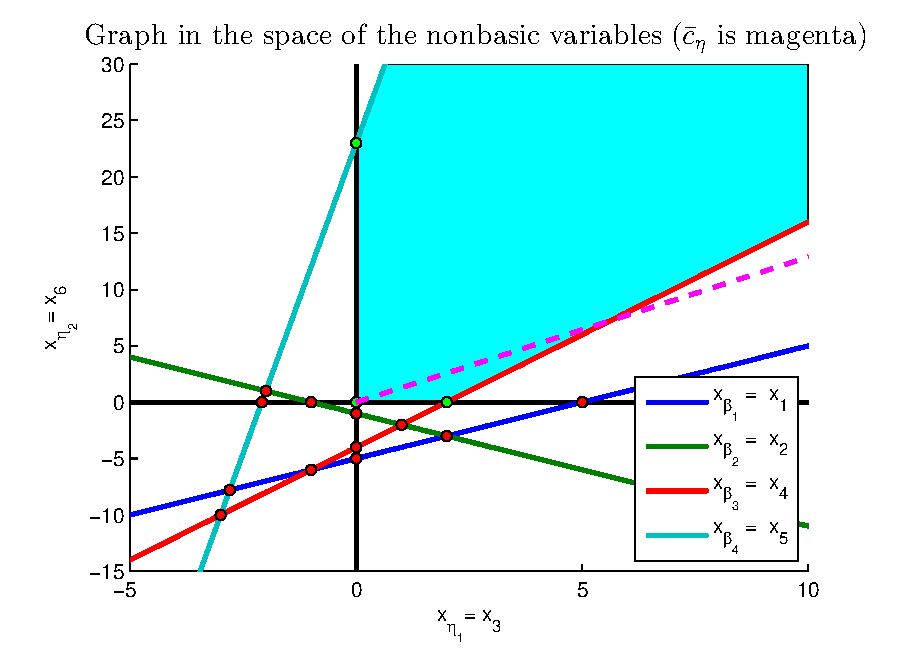
\includegraphics[width=0.7\textwidth]{p1/p1.eps}
\caption{Feasible region projected into the space of $(x_3,x_6)$}\label{fig:p1}
\end{figure}

\begin{table*}[!h]
\centering
\footnotesize
\begin{tabular}{|c|c|c|c|c|c|}\hline

\textbf{basic partition} & \textbf{basic feasible} & \textbf{basic (feasible)} & $\bar{A}_{\eta_j}$ & $ \bar{b} := A_{\beta}^{-1}b$ & $\bar{\lambda}$ \\
&\textbf{solution} & \textbf{direction} & & & \\
\hline
$\beta = (1,2,4,6) $, $\eta = (3,5)$&(14,4,0,9,0,23)'&(5,2,1,3,0,11)'& (-5,-2,-3,-11)' &(14,4,9,23)'&$\to+\infty$\\
&&(-3,-1,0,-2,1,-6)'& (3,1,2,6)'&&23/6\\\hline
$\beta = (1,2,4,5) $, $\eta = (3,6)$&(2.5,1/6,0,4/3,23/6,0)'&(-0.5,1/6,1,-2/3,11/6,0)'& (0.5,-1/6,2/3,-11/6)' &(2.5,1/6,4/3,23/6)'&2\\
&&(0.5,1/6,0,1/3,-1/6,1)'& (-0.5,-1/6,-1/3,1/6)' &&23\\\hline
$\beta = (1,2,3,5) $, $\eta = (4,6)$&(1.5,0.5,2,0,7.5,0)'&(0.75,-0.25,-1.5,1,-2.75,0)'& (-0.75, 0.25,1.5,2.75)' &(1.5,0.5,2,7.5)'&4/3\\
&&(0.25,0.25,0.5,0,0.75,1)'& (-0.25,-0.25,-0.5,-0.75)' &&$\to+\infty$\\\hline
\end{tabular}
\caption{Basic direction, basic feasible direction and maximum step}
\label{tab:max-step}
\end{table*}

\begin{table*}[!h]
\centering
\footnotesize
\begin{tabular}{|c|c|c|c|c|c|}\hline

\textbf{basic partition} & \textbf{basic feasible} & \textbf{basic (feasible)} & $\bar{\lambda}$ & \textbf{another basic} \\
&\textbf{solution} & \textbf{direction ($\bar{z}$)} & & \textbf{feasible solution} \\
\hline
$\beta = (1,2,4,6) $, $\eta = (3,5)$&(14,4,0,9,0,23)'&(5,2,1,3,0,11)'&$\to+\infty$&-\\
&&(-3,-1,0,-2,1,-6)'&23/6&(2.5,1/6,0,4/3,23/6,0)'\\\hline
$\beta = (1,2,4,5) $, $\eta = (3,6)$&(2.5,1/6,0,4/3,23/6,0)'&(-0.5,1/6,1,-2/3,11/6,0)'&2&(1.5,0.5,2,0,7.5,0)'\\
&&(0.5,1/6,0,1/3,-1/6,1)'&23&(14,4,0,9,0,23)'\\\hline
$\beta = (1,2,3,5) $, $\eta = (4,6)$&(1.5,0.5,2,0,7.5,0)'&(0.75,-0.25,-1.5,1,-2.75,0)'&4/3&(2.5,1/6,0,4/3,23/6,0)'\\
&&(0.25,0.25,0.5,0,0.75,1)'&$\to+\infty$&-\\\hline
\end{tabular}
\caption{Another basic feasible solution}
\label{tab:another-sol}
\end{table*}

The \textbf{basic direction} and \textbf{basic feasible direction relative to the basic feasible solution} are shown in Table \ref{tab:direction}. We check whether a basic direction is a basic feasible direction by verifying  $\bar{b} = A_{\beta}^{-1}b$: $\bar{b}_i > 0$, for all $i$ such that $\bar{a}_{i,\eta_j}>0$, where $\bar{A}_{\eta_j} := A_{\beta}^{-1}A_{\eta_j}$. 

The \textbf{basic feasible rays} $\bar{z}$ are $(5,2,1,3,0,11)'$ and $(0.25,0.25,0.5,0,0.75,1)'$ as they are basic feasible directions relative to basic feasible solutions so that $A\bar{z} = \mathbf{0}$, and also $\bar{z} \geq \mathbf{0}$. Since they are basic feasible rays, they are \textbf{extreme rays} of its feasible region.